\chapter{Testing}
Testing is a substantial part of the MangaVerse web application project. Testing helps to ensure application's 
reliability, performance and correctness. To be able to conduct efficient testing process, two kind of tests are preformed.
They are JUnit testing as a structural testing and functional testing.

\section{Structural Testing}
Structural testing also with other name white-box testing is based on testing the internal structure of the working application and it 
guarantees that the methods are working as expected.JUnit testing framework is used to conduct structural testing. JUnit testing is performed by testing 
different modules of the application such as DAOs and services. With that process each methods efficiency and correctness is guaranteed. 
Some examples of JUnit testing are shown below.\\ \\

%%TODO: change the pictures with better ones
\begin{figure}[h]
    \centering
    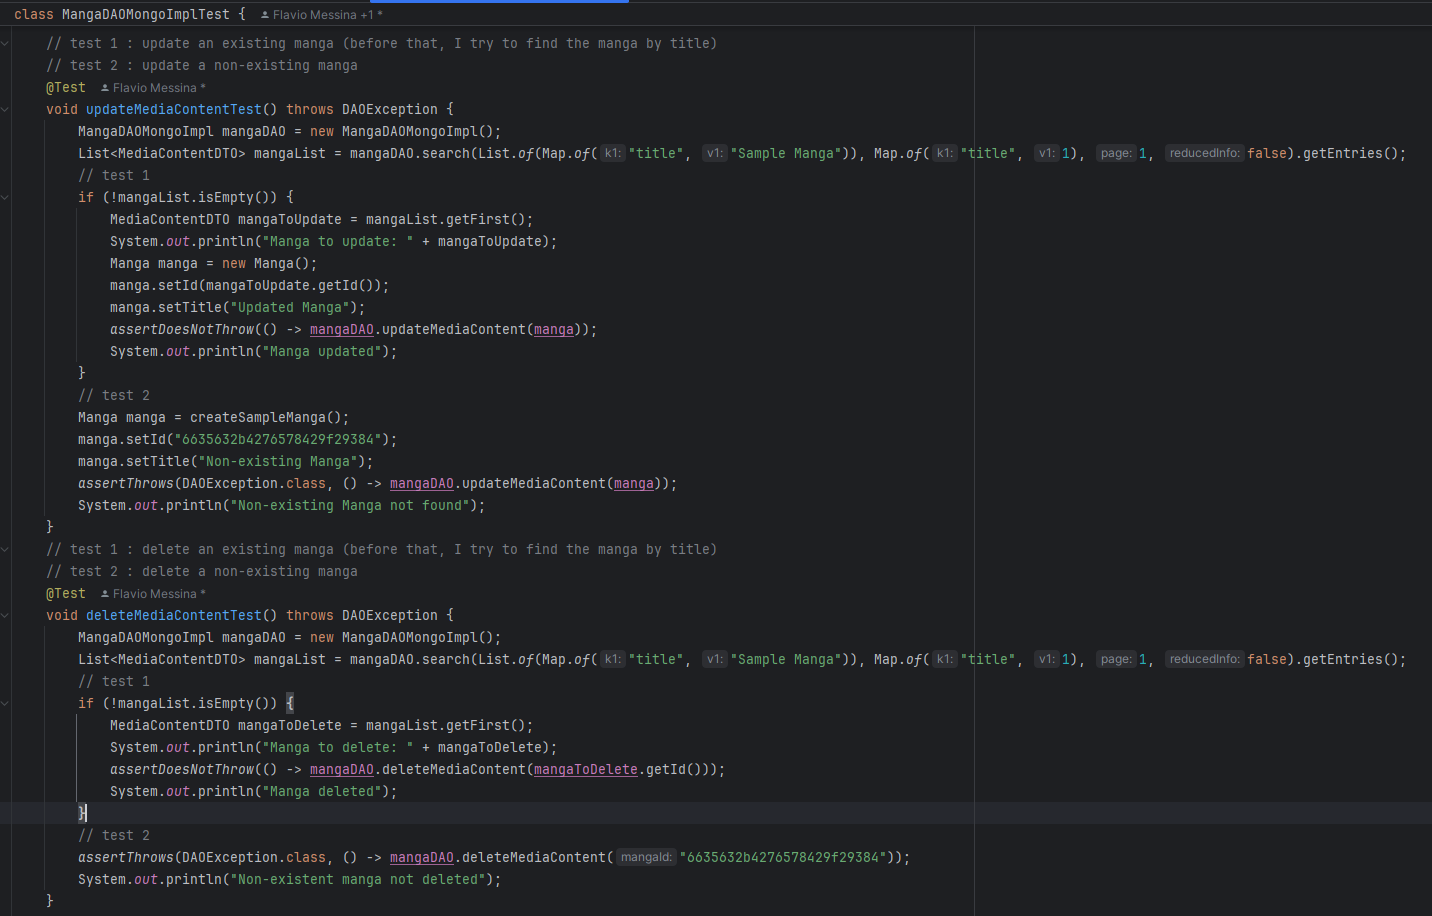
\includegraphics[width=\linewidth]{Media/test_example_1.png}
    \caption{MangaDAOMongoImpl Class Test Example}
    \label{MangaDAOMongoImpl Class Test Example}
\end{figure}

\begin{figure}[h]
    \centering
    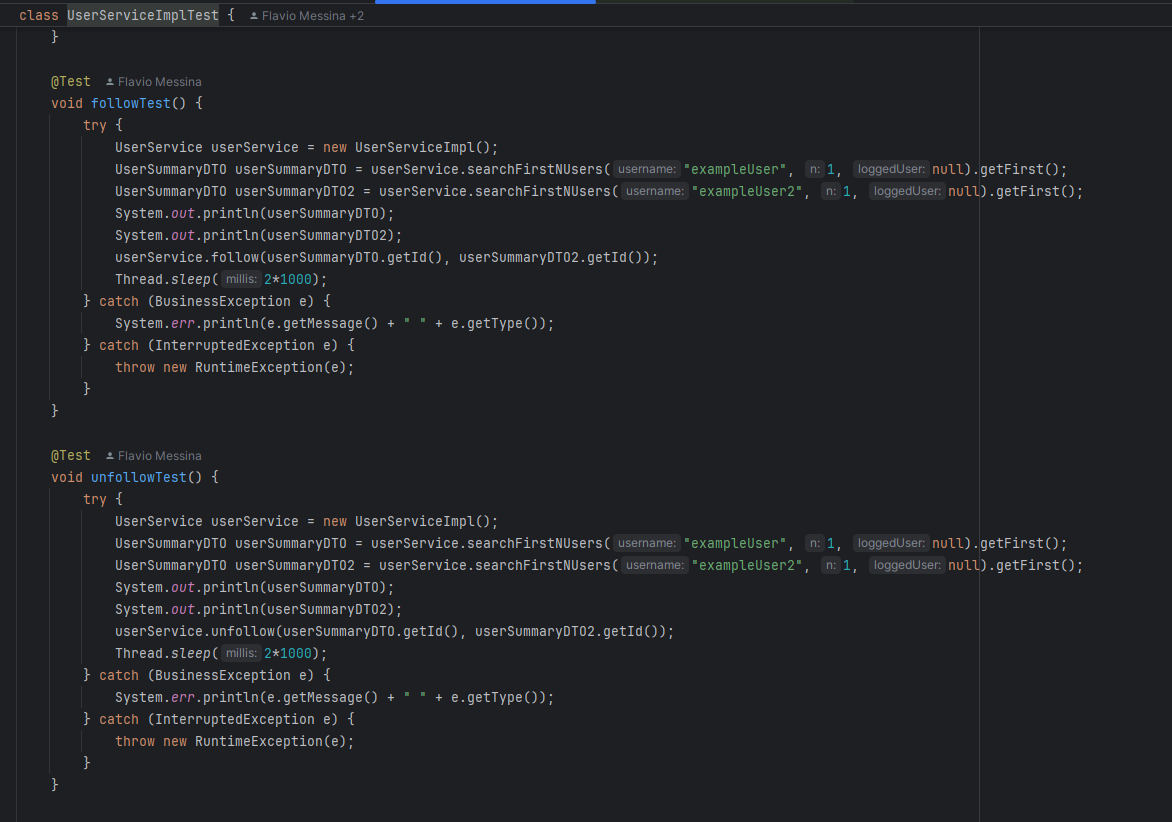
\includegraphics[width=\linewidth]{Media/test_example_2.png}
    \caption{UserServiceImpl Class Test Example}
    \label{UserServiceImpl Class Test Example}
\end{figure}

\newpage

\section{Functional Testing}
Functional testing also with other name black-box testing is based on testing the application's external functionalities. It checks the application from end-user's 
perspective. It ensures that specified requirements are provided efficiently by the web application and expected is outcome is created. 
With the help of the use cases and real world scenarios, functional testing is conducted. Some examples of functional testing are shown below.

\begin{table}[ht!]
    \centering
    \caption{Admin Test case}
    \begin{tabularx}{\textwidth}{|c|>{\RaggedRight}p{2.2cm}|>{\RaggedRight}X|>{\RaggedRight}p{2.7cm}|>{\RaggedRight}p{1.98cm}|>{\RaggedRight}p{1.5cm}|}
        \hline
        \textbf{Id} & \textbf{Description} & \textbf{Input} & \textbf{Expected Output} & \textbf{Output} & \textbf{Outcome} \\
        \hline
        User\_01 & Login with correct information & email: nmiller@example.com, password: f6d6b3ffecb44a... & The user logs in successfully &  &  \\
        \hline
        User\_02 & Login with wrong information  & email: wrong@example.com, password: wrong  & The user is not able to log in successfully &  &  \\
        \hline
        User\_03  & Signup with all the mandatory info are filled &  &  &  &  \\
        \hline
        User\_04  & Signup with missing info &  &  &  &  \\
        \hline
        User\_05 & Update user information & description: manga lover & User profile is updated with new info.  &  &  \\
        \hline
        User\_06 & Follow another user & - & User is followed.  &  &  \\
        \hline
        User\_07 & Unfollow another user & - & User is unfollowed. &  &  \\
        \hline
        User\_08 & Search manga by title & title: "Slam Dunk"  & The list of manga which includes the words of "Slam Dunk" is shown.  &  &  \\
        \hline
        User\_09 & Search manga by detailed filtering &  &  &  &  \\
        \hline
        User\_10 & Like anime & - & The anime is liked &  &  \\
        \hline
        User\_11 & Add review to anime & review:"I like the anime"  & The review is added to the anime and displayed in the anime page  &  &  \\
        \hline
        User\_12 & Update review & review: "I dont like this anime anymore" & The review is updaated with the new one. &  &  \\
        \hline
        Admin\_01 & See users distribution analytics   & - &  &  &  \\
        \hline
        Admin\_02 & See manga analytics for get average rating by month & Year:2020 & Average rating for each month in 2020 is displayed in the page &  &  \\
        \hline
        Admin\_03 & See anime analytics for get trend media content by year &  &  &  &  \\
        \hline
        Admin\_04 &  &  &  &  &  \\
        \hline
        Admin\_05 &  &  &  &  &  \\
        \hline
        %\multirow{2}{*}{A\_T\_07} & \multirow{2}{2.2cm}{Search } & Write  & \multirow{2}{\linewidth}{Show the list} & List  & Passed \\
        %\hline
        %\multirow{2}{*}{A\_T\_08} & \multirow{2}{2.2cm}{Search } & Write & \multirow{2}{\linewidth}{Show the list } & List   & Passed \\
        %\hline
    \end{tabularx}
\end{table}